%
% $Id: ch01_overview
%
%   *******************************************************************
%   * SEE THE MAIN FILE "AllegThesis.tex" FOR MORE INFORMATION.       *
%   *******************************************************************

\chapter{Introduction}\label{ch:intro} % we can refer to chapter by the label

%   ************************************************************************
%   * In LaTeX, new paragraphs are begun by simply leaving a blank line in *
%   * the LaTeX file.                                                      *
%   *                                                                      *
%   * The \\ characters should NEVER be used to end a paragraph.           *
%   * They are used only for inserting line breaks in certain situations.  *
%   *                                                                      *
%   * "Widows" (ending paragraph lines at the top of a new page) and       *
%   * "orphans" (opening paragraph lines at the bottom of a page) should   *
%   * be eliminated; this sometimes requires re-writing some of the        *
%   * text to change the line lengths.                                     *
%   ************************************************************************


\section{Importance of Energy Efficiency} \label{sec:motivation}

Energy usage globally has risen about 70 percent since 1971 and is projected to continue to rise in the future as countries across the world become more developed and have larger economies. Based on 2010 estimates, energy demand is projected to rise at over 2 per cent per year for the next 15 years if current energy usage patterns persist \cite{wri}. Rising energy use leads to an increase in greenhouse gas emissions from fossil fuels which further leads to an increase in chances of climate change. According to the World Resources Institute, about 90 percent of the world's commercial energy comes from fossil fuels, and ``energy related emissions account for more than 80 percent of the carbon dioxide (CO\textsubscript{2}) released into the atmosphere each year'' \cite{wri}. Global energy consumption and annual CO\textsubscript{2} emissions have risen by almost 50 percent from 1993 levels \cite{wri}.

Energy efficiency, i.e., delivering the same (or more) services for less energy, is one of the quickest and cheapest ways to increase the amount of energy available for use. The European Council for an Energy Efficient Economy describes energy efficiency  as the `cornerstone of a sustainable society' \cite{ecees}.A large share of the energy supply has to come from renewable energy sources such as wind and solar power in order to comply with international treaties such as the Kyoto Protocol. However, with increasing energy demand, the development of renewables needs to be supplemented with energy efficiency.

From an environmental perspective, an obvious benefit to energy efficiency is 
the reduction in the amount of greenhouse gas emissions. Reduction in greenhouse gas emissions can help with  improving urban air quality, reducing acid rain, and reducing eutrophication (i.e. an increase in the concentration of nutrients in water that promotes excessive algae growth) \cite{ecees}. There are economic benefits to energy efficiency as well. According to the Department of Energy's Energy Efficiency and Renewable Energy program, Americans saved \$7 billion on residential energy bills in 2004 from energy saving measures and by building energy efficient homes \cite{wri}. Increased energy efficiency contributes to energy security and makes a country more competitive in an increasingly globalized world. 

Buildings have an enormous impact on the environment, using about 40 percent of natural resources extracted in industrialized countries, consuming nearly 70 percent of electricity and 12 percent of potable water, and producing between 45 and 65 percent of the waste disposed in landfills. Moreover, they are responsible for a large amount of harmful emissions, accounting for 30 percent of greenhouse gases, due to their operation, and an additional 18 percent caused indirectly by material exploitation and transportation \cite{Castro-Lacouture2009}. Buildings in the United States account for about 39 percent of the total primary energy consumption and 70 percent of the electricity consumption(Fig.\ref{fig:energy})\cite{Wang2005a}. Energy efficiency in buildings can thus play an important role in making the building `green'. Some such measures are structural and can only be included in newly constructed buildings; many others can be incorporated during building refurbishment. While there are software tools available to simulate the effects and impacts of a particular design, tools for optimizing the design are not readily available \cite{Wang2005b} \cite{Pernodet2009}.

\begin{figure}[htbp]
\centering
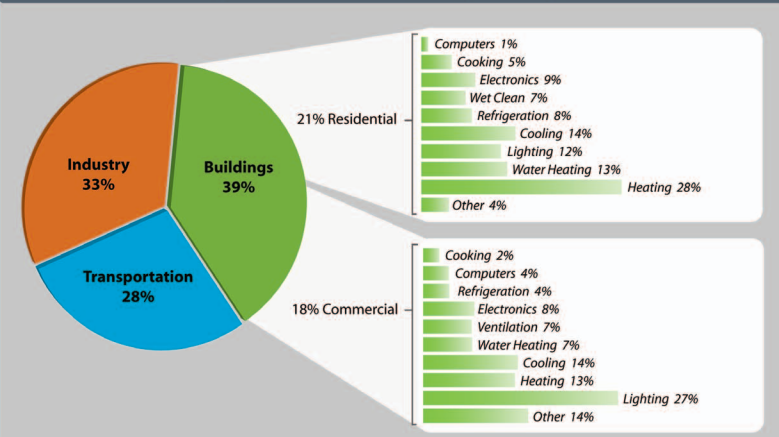
\includegraphics[width=0.8\linewidth,scale=0.6]{images/energy.png}
\caption{Buildings Share of U.S. Primary Energy Consumption 
Uses \cite{wri}}
\label{fig:energy}
\end{figure}

\section{Optimization techniques}\label{sec:stateofart}
Solving an optimization problem allows us to find at least one solution that 
minimizes or maximizes a particular criterion. This criterion is represented by an objective or a fitness function that depends on variable parameters (both continuous and discrete) that describe the solutions \cite{Pernodet2009}. 
Optimizations can be both single criterion or multi criteria. There are three 
main methods for optimization: enumerative, calculus based, and random \cite{Pernodet2009}. Enumerative methods go through every single solution in the search space in order to find the optimal one. While this method is simple, it is extremely inefficient especially when it comes to problems such as building optimization due to the huge number of possible solutions. Calculus based methods use a rigorous mathematical expression of the objective function. The main limitation to this method, besides having to know an explicit mathematical expression (that sometimes has to be continuous), is that it can find a local optimum in the neighborhood without going through the global search space. Random methods, as the name suggests, use random evaluation of solutions and are often built to emulate other phenomena.

\begin{figure}[htbp]
\centering
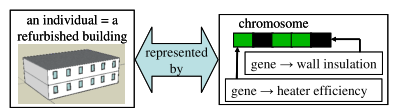
\includegraphics[width =0.7\linewidth]{images/pernodet.png}
\caption{Representing solutions as chromosome \cite{Pernodet2009}}
\label{fig:pernodet}
\end{figure}


Genetic algorithms (GAs) are a form of random optimization methods that seek to mimic the process of evolution in order to select an optimal solution. Strings of either real numbers or  bits (binary digits, 0 and 1) are used analogous to a gene in order to represent the parameters (Fig.\ref{fig:pernodet}) \cite{Pernodet2009} \cite{Coley2002}. Multiple such sub-strings are then concatenated to form the genotype. An initial population of theses genotypes is generated randomly. The algorithm consists of three main functions : selection, mutation and crossover (Fig.\ref{fig:pernodet2}). During selection, the fitness of an individual string is evaluated using the parameter values it represents. The fittest of the strings are then crossed-over i.e. allowed to mate and produce progeny by combining substrings of random length from pairs of genotypes. Mutation is allowed by occasional changing the values of a string position of a newly created progeny. After a number of generations of the process, the parameter values represented by the genotypes hopefully converge towards optimal solution values \cite{Coley2002}.

\begin{figure}[htbp]
\centering
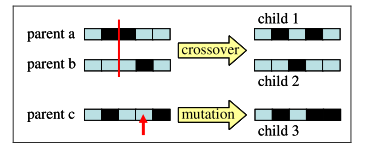
\includegraphics[width =0.7\linewidth]{images/pernodet2.png}
\caption{Crossover and Mutation operators \cite{Pernodet2009}}
\label{fig:pernodet2}
\end{figure}


The general advantages of using genetic algorithms for optimization problems are all relevant in the case of energy optimization for buildings. GAs do not 
require a knowledge of the mathematical structure of the problem. A GA search is not limited to a local optimum \cite{Pernodet2009}. Further, multi objective GAs such as the non-dominated sorting genetic algorithm (NSGA-II) produce Pareto optimal solutions. A solution is Pareto optimal if a decrease in one objective cannot happen without an increase in at least one other objective \cite{Deb2002}\cite{Pernodet2009}. For a problem with two objectives (such as energy consumption and cost), the result is a curve of Pareto solutions instead of just one solution. Thus, this allows us to obtain a whole set of solutions from which we can then choose (Fig.\ref{fig:pareto}). %Add more about MOGA%

\begin{figure}[htbp]
\centering
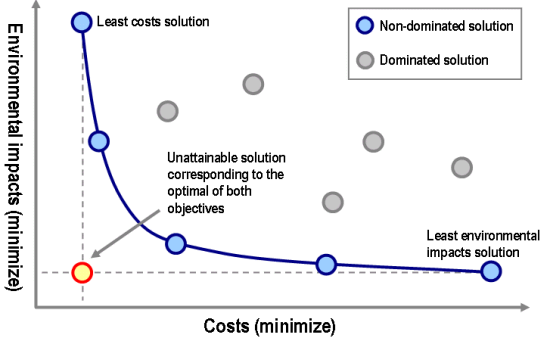
\includegraphics[width = 0.5\linewidth]{images/pareto.png}
\caption{Pareto Optimal Solution Curve \cite{Coley2002}}
\label{fig:pareto}
\end{figure}

\section{Goals of the Project}\label{sec:goals}

The aim of this proposed project is to use a genetic algorithm based approach 
to create a system for optimizing energy efficiency in a building. The system 
will take in parameters needed to model the building design and output a set of Pareto optimal solutions. This will be a multi-objective optimization problem with two objectives\textemdash minimizing energy usage and minimizing associated cost. A multi-objective genetic algorithm, NSGA-II will be used along with a building energy simulation program, EnergyPlus for fitness evaluation. The following chapters outline genetic algorithm and the NSGA-II algorithm in details, discuss some related work in the field and explain the method of approach. I will also present the results of a case study of the system using Alden Hall, a building on Allegheny College campus. Finally, I will discuss the results of the case study in context of other related work in the area.


% COMMENTED OUT NEXT FEW LINES TO SAVE SPACE; MAY PUT THEM BACK LATER
%Following the concise statement of the thesis, some of the details can be
%expanded.  
%It is appropriate to
%refer to some of the results in the introduction (which may 
%mean going back and adding them to the introduction once the
%research is completed). 
%A senior thesis, or any research paper, is not a mystery 
%novel---there is no need to keep the reader in suspense about what
%has been accomplished.

% \section{Thesis Outline}\label{sec:outline}
% The introductory chapter usually concludes with a ``road map'' of the upcoming
% chapters, e.g., ``Chapter \ref{ch:relatedwork} reviews a number of past approaches
% to the problem and summarizes their strengths and weaknesses. Chapter 
% \ref{ch:method} outlines the method of approach used to establish the
% results.''
